\section{Polar Coordinates}

\subsection{Definition}

In a rectangular coordinate system, every point in space can be represented by a list of two numbers: the x-coordinate and the y-coordinate of the point.  Put another way, for any point in a 2-dimensional space, we can represent that point by the tuple $(x,y)$.  A {\bf tuple} is an ordered list of numbers.\\

It is also possible to represent every point in a 2-dimensional space using angles.  Let us choose some point in space.  Make a line between this point and the origin (this figure should look familiar).  The length $r$ of the line, and the angle $\theta$ of the line contain enough information to identify that point in space.  Put another way, for any point in a 2-dimensional space, we can represent that point by the tuple $(r,\theta)$.  This is the {\bf polar coordinate system}, where every point is represented by a distance and an angle instead of an x and a y.\\

\begin{figure}[htb]
\center
\caption{Rectangular and polar coordinates.}
\label{fig:rectangular and polar coordinates}
\begin{tikzpicture}[inner sep=0pt,minimum size=0mm]
\node at (0,4.5) {};

\PAXES{0}{0}{4}{3.25}
\LANGLE{0,0}{4}{0}{45}{$\theta$}

\node at (-0.25,1.5) {$y$};
\draw[dotted] (0,4*0.7071) -- (4*0.7071,4*0.7071);
\draw[very thick,->] (0,0) -- (0,4*0.7071);

\node at (1.5,-0.25) {$x$};
\draw[dotted] (4*0.7071,0) -- (4*0.7071,4*0.7071);
\draw[very thick,->] (0,0) -- (4*0.7071,0);

\node at (1.5,1.8) {$r$};

\node at (4, 3.5) {rectangular: $(x,y)$};
\node at (4, 3) {polar: $(r,\theta)$};

\end{tikzpicture}
\end{figure}

\subsection{Polar to rectangular}

Converting polar coordinates to rectangular coordinates is simple using sines and cosines.  By definition, \\

\tab$sin(\theta) = \frac{y}{r}$  \ \ \ and \ \ \  $cos(\theta)=\frac{x}{r}$\\

Through rearrangement,\\

\tab$y = rsin(\theta)$ \ \ \ and \ \ \ $x = rcos(\theta)$

\begin{figure}[htb!]
\center
\caption{Polar coordinates to rectangular coordinates.}
\label{fig:Polar coordinates to rectangular coordinates.}
\begin{tikzpicture}[inner sep=0pt,minimum size=0mm]
\node at (0,4) {};

\PAXES{0}{0}{4}{3.25}
\LANGLE{0,0}{4}{0}{45}{$\theta$}

\node at (-0.75,1.5) {$r sin(\theta)$};
\draw[dotted] (0,4*0.7071) -- (4*0.7071,4*0.7071);
\draw[very thick,->] (0,0) -- (0,4*0.7071);

\node at (1.5,-0.25) {$r cos(\theta)$};
\draw[dotted] (4*0.7071,0) -- (4*0.7071,4*0.7071);
\draw[very thick,->] (0,0) -- (4*0.7071,0);

\node at (1.5,1.8) {$r$};

\end{tikzpicture}
\end{figure}

\subsection{Rectangular to polar}

Converting rectangular coordinates is also simple.  Using the Pythagorean theorem, \\

\tab$r = \sqrt{x^2 + y^2}$\\

and using our results from deriving inverse trigonometric functions, \\

\tab$\theta = arcsin(\frac{y}{r})$ \ \ or \ \ $\theta = arccos(\frac{x}{r})$ \ \ or \ \ $\theta = arctan(\frac{y}{x})$

\begin{figure}[htb!]
\center
\caption{Rectangular coordinates to polar coordinates.}
\label{fig:Rectangular coordinates to polar coordinates.}
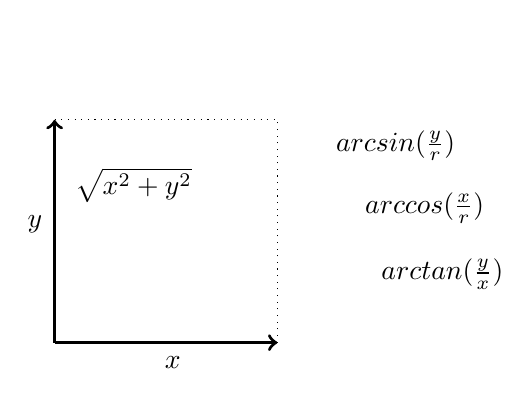
\begin{tikzpicture}[inner sep=0pt,minimum size=0mm]
\node at (0,4) {};

\PAXES{0}{0}{4}{3.25}
\LANGLE{0,0}{4}{0}{45}{}
\node at (30:5) {$arcsin(\frac{y}{r})$};
\node at (20:5) {$arccos(\frac{x}{r})$};
\node at (10:5) {$arctan(\frac{y}{x})$};

\node at (-0.25,1.5) {$y$};
\draw[dotted] (0,4*0.7071) -- (4*0.7071,4*0.7071);
\draw[very thick,->] (0,0) -- (0,4*0.7071);

\node at (1.5,-0.25) {$x$};
\draw[dotted] (4*0.7071,0) -- (4*0.7071,4*0.7071);
\draw[very thick,->] (0,0) -- (4*0.7071,0);

\node at (1,2) {$\sqrt{x^2+y^2}$};

\end{tikzpicture}
\end{figure}

\subsection{Review}

\begin{enumerate}

\item{Write the conversions from rectangular to polar coordinates, and the conversions from polar to rectangular coordinates, until you've committed them to memory.}\\

\item{Convert the following coordinates from polar to rectangular:}\\

\tab a) $(1,0^c)$\\

\tab b) $(2,\frac{\pi}{4}^c)$\\

\tab c) $(1,115^o)$\\

\tab d) $(2,-30^o)$\\

\tab e) $(0,0^o)$\\

\item{Convert the following coordinates from rectangular to polar:}\\

\tab a) $(1,0)$\\

\tab b) $(1,1)$\\

\tab c) $(0,1)$\\

\tab d) $(2,3)$\\

\tab e) $(0,0)$\\

\end{enumerate}

